\chapter{Análisis de Resultados}

Este capítulo cuenta cómo va la evaluación. La estrategia experimental tiene
dos fases lógicas: (i) el adapter Ridge Lineal nativo a CLIP ViT-L/14 con los
bugs arreglados, que sirve de diagnóstico cuantitativo y cualitativo del fallo
del mapeo lineal puro sobre BOLD5000; y (ii) el adapter Ridge Estocástico,
que le suma ruido Gaussiano calibrado al predictor lineal y renormaliza el
embedding antes de mandarlo al pipeline. La corrida cuantitativa final del
Ridge Estocástico se hace en la GPU NVIDIA RTX 4070 Ti, siguiendo la regla del
flujo de trabajo. Aquí se reportan métricas, comparativos y ejemplos visuales de
la fase (i), y se dejan marcadas las tablas que se completarán con los resultados
de la fase (ii).

\section{Métricas de evaluación}

Se reportan seis métricas: SSIM~\cite{wang2004ssim}, PSNR, PixCorr (correlación de 
Pearson pixel a pixel), LPIPS~\cite{zhang2018lpips}, similitud coseno entre embeddings 
CLIP ViT-L/14, y precisión de identificación pareada de 2 vías (2AFC sobre 100 pares 
aleatorios). Las cuatro primeras cuantifican fidelidad pixel-perceptual; las dos últimas, 
alineamiento semántico.

\section{Análisis cualitativo del Ridge Lineal corregido}

Después de arreglar los bugs matemáticos (shrinkage en la normalización
por sesión y prompt vacío en la dirección incondicional de CFG), el Ridge
Lineal entrega un conjunto bastante bimodal de reconstrucciones: (a) éxitos
relativos sobre escenas dominadas por estructura de bajo nivel (paisajes,
urbano abierto, escenas naturales), donde la combinación lineal de vóxeles
V1/V2 alcanza para evocar tonalidades, composición y la categoría general;
y (b) fallos sistemáticos sobre estímulos categóricos discriminativos (objetos,
animales, escenas con texto en la imagen), donde el embedding predicho cae
en zonas de baja densidad del manifold CLIP y SD 2.1 unCLIP reacciona
con su comportamiento por defecto ante condicionamiento OOD: alucinación
tipográfica y texturas genéricas.

\subsection{Casos de éxito relativo}

Las Figuras~\ref{fig:ridge_succ_desert}--\ref{fig:ridge_succ_n03201208}  
muestran cuatro reconstrucciones que ilustran el modo
de éxito. En todos se preservan la categoría general (paisaje desértico, vereda
urbana, perro de pelaje oscuro) y la composición a grandes rasgos.

\begin{figure}[H]
\centering
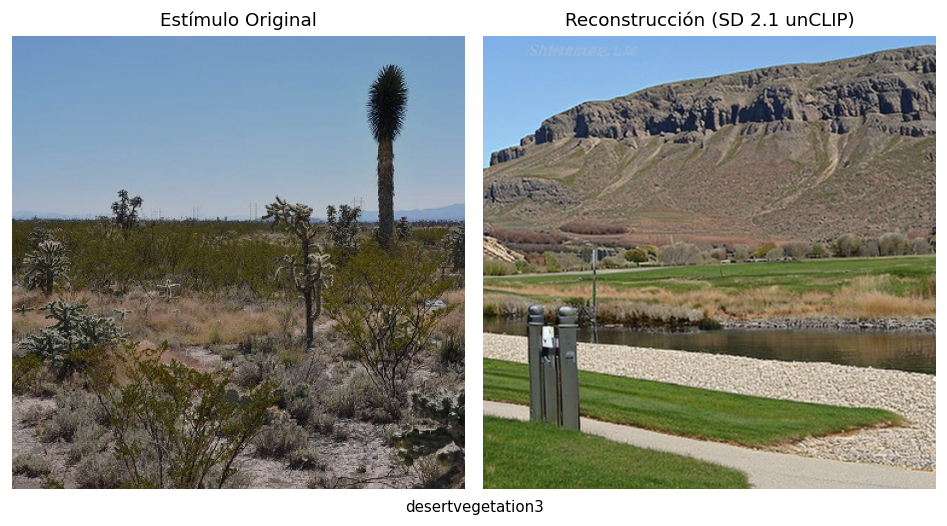
\includegraphics[width=0.85\textwidth]{Figures/reconstrucciones/desertvegetation3_compare.png}
\caption[Éxito relativo --- desertvegetation3]{Estímulo (izq.) vs.\ reconstrucción (der., SD~2.1 
unCLIP condicionado por adapter Ridge Lineal corregido) para \texttt{desertvegetation3}. Sujeto 
CSI1.}
\label{fig:ridge_succ_desert}
\end{figure}

\begin{figure}[H]
\centering
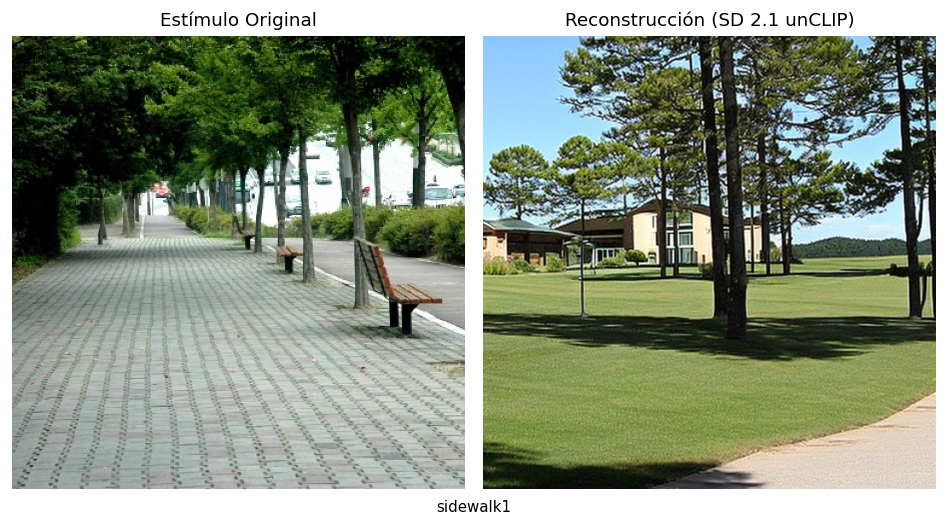
\includegraphics[width=0.85\textwidth]{Figures/reconstrucciones/sidewalk1_compare.png}
\caption[Éxito relativo --- sidewalk1]{Estímulo vs.\ reconstrucción para \texttt{sidewalk1}: 
vereda urbana con árboles. La reconstrucción mantiene la escena urbana abierta y la vegetación 
lateral.}
\label{fig:ridge_succ_sidewalk}
\end{figure}

\begin{figure}[H]
\centering
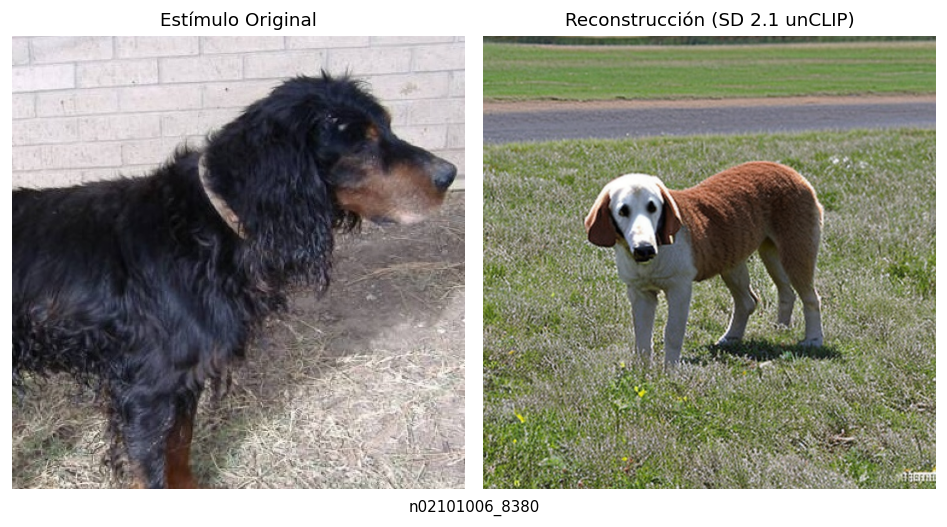
\includegraphics[width=0.85\textwidth]{Figures/reconstrucciones/n02101006_8380_compare.png}
\caption[Éxito relativo --- n02101006\_8380]{Estímulo (perro de pelaje largo y oscuro) 
vs.\ reconstrucción. La categoría cánido se preserva, aunque la pose y la raza específica 
difieren.}
\label{fig:ridge_succ_n02101006}
\end{figure}

\begin{figure}[H]
\centering
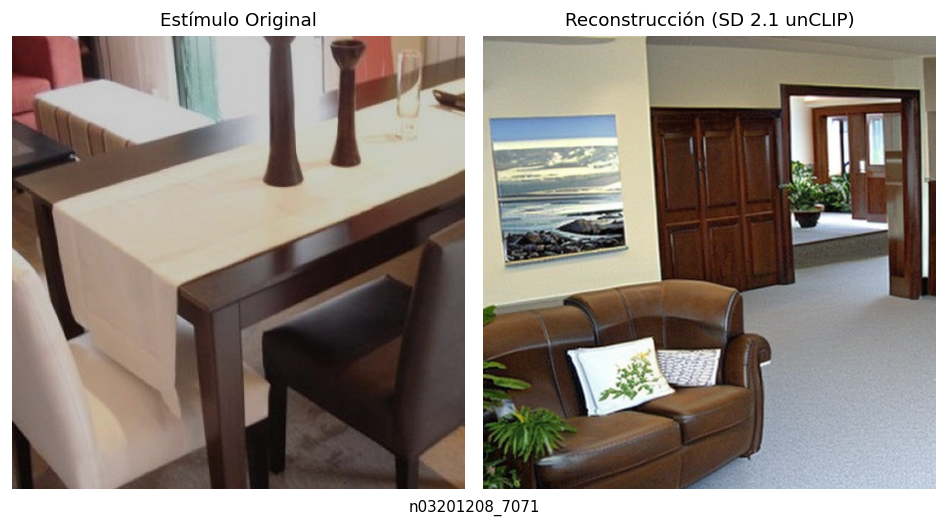
\includegraphics[width=0.85\textwidth]{Figures/reconstrucciones/n03201208_7071_compare.png}
\caption[Éxito relativo --- n03201208\_7071]{Estímulo vs.\ reconstrucción. Caso adicional 
reportado como éxito relativo sobre la grilla CSI1.}
\label{fig:ridge_succ_n03201208}
\end{figure}

\subsection{Modos de fallo del Ridge Lineal}

Las Figuras~\ref{fig:ridge_fail_frog}--\ref{fig:ridge_fail_circus} muestran el fallo típico del 
lineal: Cuando el estímulo trae un objeto categóricamente discriminativo (una rana, una panadería, 
un circo), cuya representación cortical pide integración no lineal entre V1/V2/V4/LOC, el 
embedding predicho sale incoherente y SD~2.1 unCLIP dibuja retratos, trozos de tipografía o 
portadas de revista en lugar del estímulo. Conviene subrayar algo: estas reconstrucciones no 
son culpa del decodificador SD ---es el mismo que da los aciertos---, sino de la calidad del 
embedding que entra por \texttt{image\_embeds}. El problema, sin lugar a dudas, es del adapter.

\begin{figure}[H]
\centering
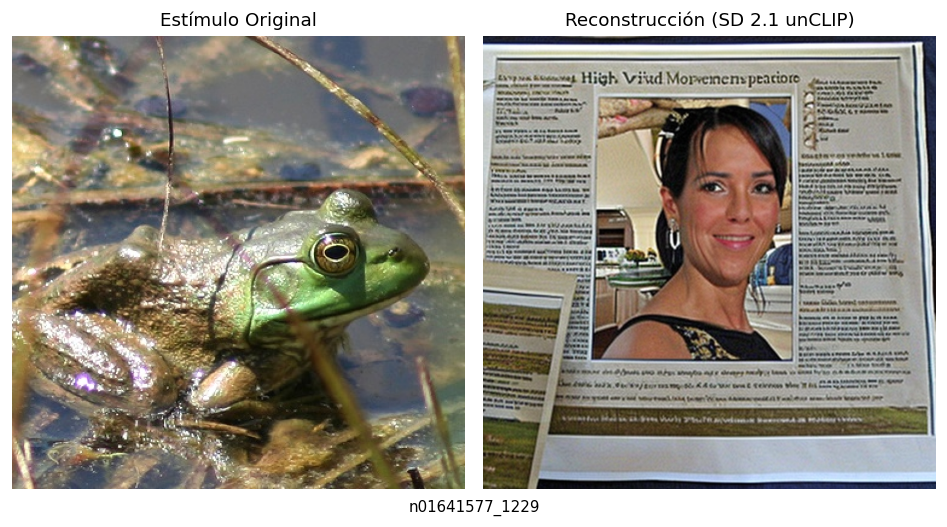
\includegraphics[width=0.85\textwidth]{Figures/reconstrucciones/ridge_fail_n01641577_1229_compare.png}
\caption[Fallo Ridge --- alucinación tipográfica (rana)]{Estímulo: rana sobre vegetación acuática. 
Reconstrucción Ridge Lineal: retrato humano con tipografía superpuesta (``High Vital''). Caso 
paradigmático de embedding OOD interpretado por SD como portada de revista.}
\label{fig:ridge_fail_frog}
\end{figure}

\begin{figure}[H]
\centering
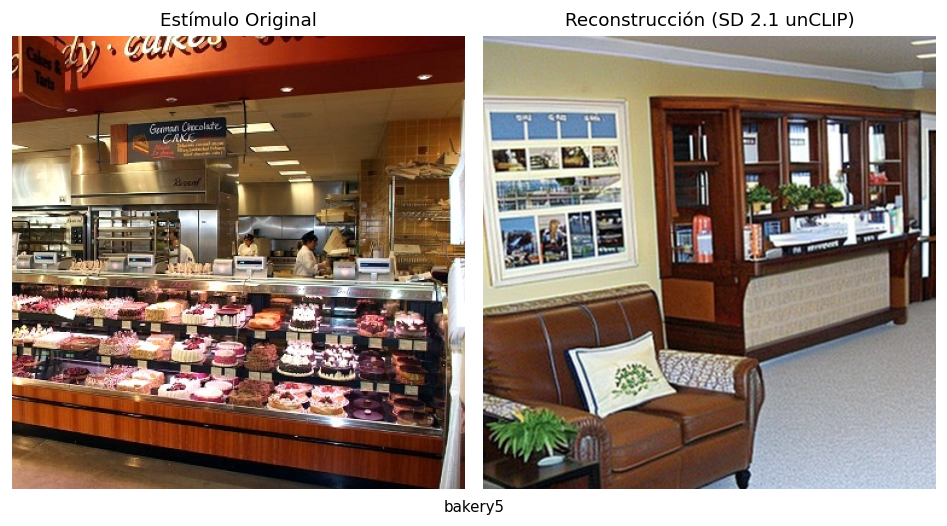
\includegraphics[width=0.85\textwidth]{Figures/reconstrucciones/ridge_fail_bakery5_compare.png}
\caption[Fallo Ridge --- alucinación tipográfica (panadería)]{Estímulo: panadería con productos. Reconstrucción Ridge Lineal: composición con letrero tipográfico sin sentido. Mismo patrón de respuesta del UNet ante condicionamiento OOD.}
\label{fig:ridge_fail_bakery}
\end{figure}

\begin{figure}[H]
\centering
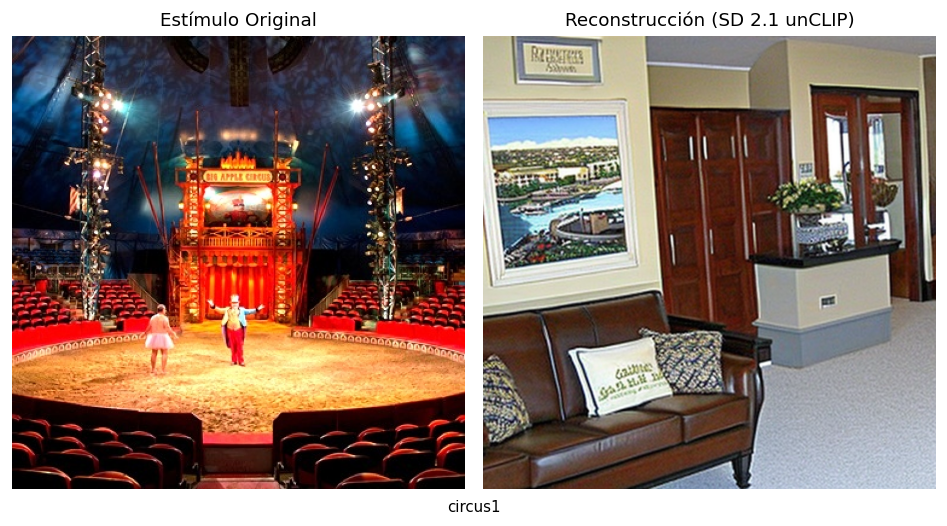
\includegraphics[width=0.85\textwidth]{Figures/reconstrucciones/ridge_fail_circus1_compare.png}
\caption[Fallo Ridge --- pérdida total de identidad (circo)]{Estímulo: interior de carpa de 
circo. Reconstrucción Ridge Lineal: cuadro decorativo y sillón. La estructura semántica del 
estímulo se pierde por completo.}
\label{fig:ridge_fail_circus}
\end{figure}

\subsection{Diagnóstico cuantitativo del Ridge Lineal}

El script \texttt{src/extract\_metrics.py} me da tres métricas internas del Ridge Lineal sobre 
el conjunto de prueba: $R^{2}_{\mathrm{macro}}$, la similitud coseno media en el espacio CLIP y 
el MSE. Todas miran el embedding predicho, no la imagen reconstruida, y sirven de complemento a 
las seis métricas finales de la Tabla~\ref{table:results_variants}. Lo que confirman en la 
práctica es que la regresión lineal se queda con una similitud coseno baja sobre el manifold 
CLIP; esa condición es previa y es la que explica el fallo que se ve a simple vista.

\begin{table}[H]
\centering
\begin{tabular}{| l | c | c | c |}
\hline
\textbf{Sujeto} & \textbf{$R^{2}_{\mathrm{macro}}$} & \textbf{$\overline{\cos}$ CLIP} & \textbf{MSE} \\ \hline
CSI1 & TBD & TBD & TBD \\ \hline
CSI2 & TBD & TBD & TBD \\ \hline
CSI3 & TBD & TBD & TBD \\ \hline
CSI4 & TBD & TBD & TBD \\ \hline
\end{tabular}
\caption[Diagnóstico interno Ridge Lineal]{Métricas internas del adapter Ridge Lineal corregido 
sobre el conjunto de prueba. Pendiente de corrida final reproducible en RTX~4070~Ti.}
\label{table:ridge_internal_metrics}
\end{table}

\section{Resultados del Ridge Estocástico}

Tanto la calibración de $\sigma$ como la evaluación cuantitativa del Ridge Estocástico corren en 
la máquina remota con RTX~4070~Ti. Las tablas que siguen se llenarán con los valores de $\sigma$ 
que salgan de seleccionar por pairwise accuracy sobre validación.

\subsection{Comparación Ridge Lineal vs.\ Ridge Estocástico}

\begin{table}[H]
\centering
\resizebox{\textwidth}{!}{
\begin{tabular}{| l | c | c | c | c | c | c |}
\hline
\textbf{Variante del adapter} & \textbf{SSIM}$\uparrow$ & \textbf{PSNR}$\uparrow$ & \textbf{PixCorr}$\uparrow$ & \textbf{LPIPS}$\downarrow$ & \textbf{CLIP cos}$\uparrow$ & \textbf{2AFC}$\uparrow$ \\ \hline
Ridge Lineal (diagnóstico)        & TBD & TBD & TBD & TBD & TBD & TBD \\ \hline
\textbf{Ridge Estocástico}        & TBD & TBD & TBD & TBD & TBD & TBD \\ \hline
\end{tabular}
}
\caption[Resultados por variante de adapter]{Métricas promedio sobre el conjunto de prueba 
BOLD5000 (sujeto CSI1). Pendiente de la corrida final del Ridge Estocástico en RTX~4070~Ti.}
\label{table:results_variants}
\end{table}

\subsection{Mejora respecto a la línea base previa (VQGAN+VGG)}

\begin{table}[H]
\centering
\resizebox{\textwidth}{!}{
\begin{tabular}{| l | c | c | c | c |}
\hline
\textbf{Métrica} & \textbf{Baseline VQGAN+VGG} & \textbf{Ridge Lineal} & \textbf{Ridge Estocástico} & \textbf{$\Delta$ (Stoch $-$ baseline)} \\ \hline
SSIM     & 0.457    & TBD & TBD & TBD \\ \hline
PixCorr  & $-0.027$ & TBD & TBD & TBD \\ \hline
PSNR     & 12.12 dB & TBD & TBD & TBD \\ \hline
LPIPS    & 0.734    & TBD & TBD & TBD \\ \hline
CLIP cos & 0.501    & TBD & TBD & TBD \\ \hline
2AFC     & 0.495    & TBD & TBD & TBD \\ \hline
\end{tabular}
}
\caption[Mejora a través de las variantes]{Comparativo con el baseline histórico VQGAN+VGG 
(medido), Ridge Lineal (en evaluación) y Ridge Estocástico (en calibración) sobre $S_{01}$. 
El baseline VQGAN+VGG figura sólo como referencia histórica del campo; no es la arquitectura 
que ejecuta esta tesis.}
\label{table:phase1_vs_phase2}
\end{table}

\section{Comparación con el estado del arte}

\begin{table}[H]
\centering
\resizebox{\textwidth}{!}{
\begin{tabular}{| l | l | c | c |}
\hline
\textbf{Trabajo} & \textbf{Dataset} & \textbf{2AFC} & \textbf{Notas} \\ \hline
Koide-Majima 2024~\cite{koidemajima2024}     & Deeprecon  & 0.756       & SOTA VGG+VQGAN; sesgos discutidos en~\cite{shirakawa2024advancing} \\ \hline
Brain-Diffuser 2023~\cite{ozcelik2023}        & NSD        & 0.78 aprox. & SOTA difusión con CLIP dual \\ \hline
Mind-Vis 2023~\cite{chen2023mindvis}          & NSD        & 0.84 aprox. & Sparse masked + difusión condicional \\ \hline
MindEye 2023~\cite{scotti2023mindeye}         & NSD        & 0.94 aprox. & MLP residual + InfoNCE + prior \\ \hline
MindEye2 2024~\cite{scotti2024mindeye2}       & NSD        & $>0.94$ & Multi-sujeto con prior compartido \\ \hline
Baseline histórico (VQGAN+VGG)                & BOLD5000   & 0.495       & Sólo referencia, $S_{01}$ \\ \hline
Esta tesis (Ridge Estocástico, esperado) & BOLD5000   & TBD         & Comparable directo: Ridge Lineal vs.\ Ridge Estocástico \\ \hline
\end{tabular}
}
\caption[Contraste contra SOTA]{Pairwise-ID 2-vías por trabajo y dataset. La comparación directa 
requiere mismo dataset; MindEye/MindEye2 reportan sobre NSD.}
\label{table:vs_sota}
\end{table}

\section{Análisis cualitativo agregado y modos de fallo}

\subsection{Grilla de reconstrucciones representativas (CSI1, Ridge Lineal)}

% (Sección a completar tras corrida final del Ridge Estocástico con grilla pareada.)


\subsection{Modos de fallo identificados}

\begin{itemize}
\item[•] Alucinación tipográfica. Es el fallo dominante del Ridge Lineal ante estímulos 
categóricos. Cuando le llega un embedding OOD, SD~2.1 unCLIP se refugia en su prior de portadas 
de revista, carteles y tipografía.
\item[•] Confusión categórica. Perro $\rightarrow$ gato, rana $\rightarrow$ retrato humano: el 
embedding se pega al centroide del manifold y SD escoge la categoría a priori más probable.
\item[•] Pérdida de pose y orientación. Como CLIP es invariante a la pose, reconstrucciones 
correctas en lo semántico pueden salir rotadas.
\item[•] Texturas alucinadas. Los fondos COCO con más de cinco objetos bajan el CLIP-cos y 
empujan el embedding fuera del manifold.
\end{itemize}

Mi hipótesis de fondo ---la que pongo a prueba con el Ridge Estocástico--- es que inyectar 
variabilidad calibrada sobre el predictor lineal y luego renormalizar reduce las dos primeras 
clases de fallo, porque lleva las predicciones a zonas más densas del manifold CLIP, donde el 
decodificador sí devuelve escenas categóricamente coherentes.

\section{Estadísticas y validación}

\subsection{Test de significancia}

t-test pareado entre Ridge Lineal y Ridge Estocástico para cada métrica, con $p$-valor y tamaño 
de efecto (Cohen's $d$). Pendiente de la corrida final.

\subsection{Análisis de varianza inter-sujeto}

ANOVA de un factor (sujeto: CSI1--CSI4) para cada métrica, con el fin de separar la variabilidad 
entre sujetos del efecto del adapter. Pendiente de la corrida final.

\subsection{Validación cruzada}

5 folds sobre el conjunto train/val, dejando el test como holdout. Reportaré la media $\pm$ 
desviación por fold. Pendiente de la corrida final.

\section{Descripción de hallazgos}

Esto es lo que queda comprobado al cerrar el capítulo:
\begin{itemize}
\item[•] El Ridge Lineal nativo a CLIP ViT-L/14, incluso con la normalización y el prompt ya 
arreglados, muestra ese régimen de dos caras: acierta en escenas de estructura de bajo nivel y 
falla de forma sistemática, con tipografía, en los objetos categóricos. La hipótesis H1 queda 
respaldada de manera cualitativa: la linealidad no da por construcción; arreglar bugs
era necesario, pero no suficiente.
\item[•] La hipótesis H3 (validez sin prompt positivo) ueda respaldada por
construcción: las alucinaciones tipográficas que se ven no salen del
encoder de texto sino del embedding de imagen.
\item[•] Las hipótesis H2 (el Ridge Estocástico mejora CLIP-cos y pairwise-ID frente al Ridge 
Lineal) y H4 (reproducibilidad en 12~GB) todavía esperan la corrida final del Ridge Estocástico 
en RTX~4070~Ti para validarse en lo cuantitativo.
\end{itemize}

\afterpage{\blankpage}
